\documentclass[12pt]{exam}
%\printanswers


\setlength{\parindent}{0pt}
\setlength{\parskip}{.25cm}

\usepackage{graphicx}

\usepackage{xcolor}

\definecolor{darkred}{rgb}{0.5,0,0}
\definecolor{darkgreen}{rgb}{0,0.5,0}
\usepackage{hyperref}
\hypersetup{
  letterpaper,
  colorlinks,
  linkcolor=red,
  citecolor=darkgreen,
  menucolor=darkred,
  urlcolor=blue,
  pdfpagemode=none,
  pdftitle={CSCE 156 Lab Handout},
  pdfauthor={Christopher M. Bourke},
  pdfsubject={},
  pdfkeywords={}
}

\definecolor{MyDarkBlue}{rgb}{0,0.08,0.45}
\definecolor{MyDarkRed}{rgb}{0.45,0.08,0}
\definecolor{MyDarkGreen}{rgb}{0.08,0.45,0.08}

\definecolor{mintedBackground}{rgb}{0.95,0.95,0.95}
\definecolor{mintedInlineBackground}{rgb}{.90,.90,1}

%\usepackage{newfloat}
\usepackage[newfloat=true]{minted}
\setminted{mathescape,
               linenos,
               autogobble,
               frame=none,
               framesep=2mm,
               framerule=0.4pt,
               %label=foo,
               xleftmargin=2em,
               xrightmargin=0em,
               startinline=true,  %PHP only, allow it to omit the PHP Tags *** with this option, variables using dollar sign in comments are treated as latex math
               numbersep=10pt, %gap between line numbers and start of line
               style=default, %syntax highlighting style, default is "default"
               			    %gallery: http://help.farbox.com/pygments.html
			    	    %list available: pygmentize -L styles
               bgcolor=mintedBackground} %prevents breaking across pages
               
\setmintedinline{bgcolor={mintedBackground}}
\setminted[text]{bgcolor={mintedBackground},linenos=false,autogobble,xleftmargin=1em}
%\setminted[php]{bgcolor=mintedBackgroundPHP} %startinline=True}
\SetupFloatingEnvironment{listing}{name=Code Sample}
\SetupFloatingEnvironment{listing}{listname=List of Code Samples}


\title{CSCE 156 -- Computer Science II \\
{\large Lab 8.0 - SQL II - Worksheet}}
\author{~}
\date{~}

\begin{document}

\maketitle

{\Large Names \underline{\hspace*{5cm}}}

For each question, write an SQL query to get the specified result.  You are highly 
encouraged to use a GUI SQL tool such as MySQL Workbench and keep track of your 
queries in an SQL script so that lab instructors can verify your work.  If you do, 
write your queries in the script file provided rather than hand-writing your queries 
here.

\fullwidth{\section{Inserting \& Manipulating Data}}

\begin{questions}

\question Choose your favorite album and insert it into the database by doing 
  the following.
\begin{parts}
  \part Write a query to insert the band of the album
  \part Write a query to insert the album
  \part Write two queries to insert the first two songs of the album
  \part Write two queries to associate the two songs with the inserted album
\end{parts}

\begin{solution}

\begin{minted}{sql}
insert into Band (name) values ('The Faint');
insert into Album (title,year,number,bandId) values ('Danse Macabre',2001,5,
(select bandId from Band where name = 'The Faint'));
insert into Song (title) values ('Agenda Suicide');
insert into Song (title) values ('Glass Danse');
insert into AlbumSong (trackNumber,trackLength,albumId,songId) values (1,238,
  (select albumId from Album where title = 'Danse Macabre'),
  (select songId from song where title = 'Agenda Suicide'));
insert into AlbumSong (trackNumber,trackLength,albumId,songId) values (2,180,
  (select albumId from Album where title = 'Danse Macabre'),
  (select songId from song where title = 'Glass Danse'));
\end{minted}
\end{solution}
  
\question Update the musician record for ``P. Best'', his first name should be
``Pete''.  

\begin{solution}

\begin{minted}{sql}
update Musician set firstName = 'Pete' where musicianId = ?;
\end{minted}
\end{solution}

\question Pete Best was the Beatle's original drummer, but was fired in 1962.  
Write a query that removes Pete Best from the Beatles.

\begin{solution}

\begin{minted}{sql}
delete from BandMember where bandMemberId = ?;
\end{minted}
\end{solution}

\question Attempt to delete the song ``Big in Japan'' (by Tom Waits on the album
\emph{Mule Variations}).  Write a series of queries that will allow you to delete
the album \emph{Mule Variations}.

\begin{solution}

\begin{minted}{sql}
delete from AlbumSong 
  where albumId = (select albumId from Album where title = 'Mule Variations');
delete from Album where title = 'Mule Variations';
\end{minted}
\end{solution}

\end{questions}

\newpage

\section{Designing Tables}

In this section you will design the ER by completing the diagram in Figure 
\ref{figure:erDiagram} as instructed in the following steps. All 6 information 
items in List 1 of the handout should be supported by the resulting design.

\begin{figure}
\centering
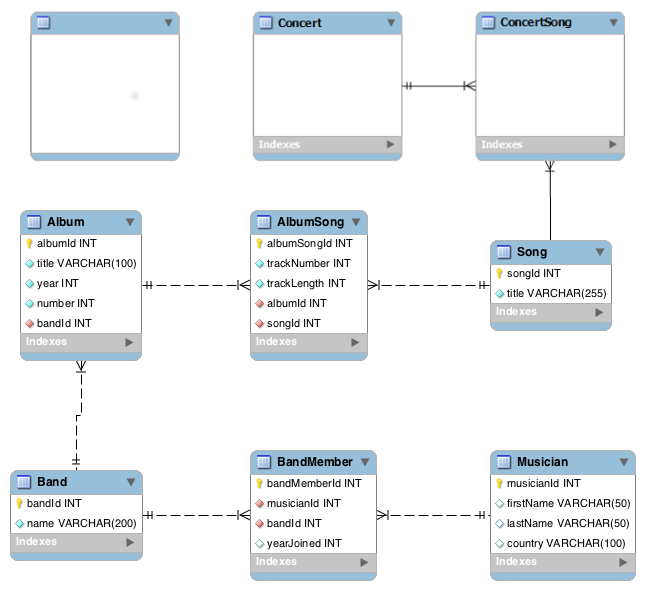
\includegraphics[scale=0.65]{images/erDiagram}
\caption{An incomplete ER diagram for the new database being designed.}
\label{figure:erDiagram}
\end{figure} 

\begin{enumerate}
  \item Use the tables from the original albums database as an example to 
    list the fields and field types associated with each of the 
    \mintinline{sql}{Concert} and \mintinline{sql}{ConcertSong} entities in 
    Figure \ref{figure:erDiagram}.  If your design needs an additional entity then 
    use the blank item. 
    
    Note: Pay attention to how the primary/foreign keys must be designed to 
    support the relations between \mintinline{sql}{Concert}, 
    \mintinline{sql}{ConcertSong} use \mintinline{sql}{BandMember} and 
    \mintinline{sql}{AlbumSong} as examples to complete \mintinline{sql}{ConcertSong}. 
    
  \item How does \mintinline{sql}{Band} from the original albums database 
    relate to the \mintinline{sql}{Concert} and/or \mintinline{sql}{ConcertSong} 
    entities? Indicate the relation(s) by drawing the appropriate line(s) onto 
    Figure \ref{figure:erDiagram} and make sure any primary/foreign keys are 
    updated to reflect this/these relation(s). 
  \item Every concert takes place at a concert hall; it is possible that the 
    name of a concert hall or its seating capacity changes. In such an event 
    your current design should not require that any previously stored concerts 
    be updated to reflect the modifications to the concert halls; if so add an 
    entity to your design to solve the problem by filling the blank item in 
    Figure \ref{figure:erDiagram}.
  \item Specify the relations between the entity you described in the blank 
    item and the other entities in Figure \ref{figure:erDiagram}. Make sure the 
    primary/foreign keys of the entities match their relations.
\end{enumerate}

\section{Create the New Tables}

Write and run a new SQL script (or simply just modify \mintinline{text}{albums.sql}) 
to generate the new tables you designed.  Alternatively, you may write a new script 
that modifies the existing database). Use Figure \ref{figure:erDiagram} as a 
blueprint for your script making sure the following items are satisfied:
\begin{itemize}
  \item Naming -- Use a uniform naming conventions for the tables and their fields
  \item Field Types -- Make sure to use appropriate types and a uniform typing conventions for each field
  \item Primary keys -- Make sure to specify which fields are primary keys
  \item Foreign keys -- Enforce appropriate foreign key restrictions to reflect each relation.
  \item Note: Some of the new relations may require you to use a 
    \mintinline{text}{alter table} statement since you may need to modify the 
    table from the original albums database design to enforce the constraints.
  \item Null/Default values -- Some entity fields are so essential that if they are 
    not provided a value the entity itself is unable to server its purpose 
    (i.e. a primary key should never be nullable). Make sure all fields are able 
    to store valid values.
\end{itemize}

Write SQL statements to do the following: 
\begin{enumerate}
  \item Write a statement to create the table \mintinline{sql}{ConcertSong}
  \item Write a statement to create the table \mintinline{sql}{Concert}
  \item Write statement(s) to create any other tables/entities that your design requires
  \item Write statement(s) to alter the original tables that you made if needed.
\end{enumerate}

\section{Using The New Tables}

You will now make sure that your design makes sense by writing several queries to insert and query data out of it.
\begin{enumerate}
  \item Write queries to insert at least two \mintinline{sql}{Concert} records.
  \item Write queries to associate at least 3 songs with each of the two concerts 
  \item Write a select-join query to retrieve these new results and produce a playlist for each concert
  \item Modify the query to include the name of the band playing the concert.  If such a query is not possible, explain why and sketch an alternative design in which it would be possible.
\end{enumerate}

\end{document}
